\documentclass[border=3pt,tikz]{standalone}
\usepackage{tikz}
\usepackage{etoolbox} % for \ifnumcomp
\usepackage{listofitems} % for \readlist to create arrays

\tikzset{>=latex} % for LaTeX arrow head
\colorlet{myred}{red!80!black}
\colorlet{myblue}{blue!80!black}
\colorlet{mygreen}{green!60!black}
\colorlet{mydarkred}{myred!40!black}
\colorlet{mydarkblue}{myblue!40!black}
\colorlet{mydarkgreen}{mygreen!40!black}
\tikzstyle{node}=[very thick,circle,draw=myblue,minimum size=22,inner sep=0.5,outer sep=0.6]
\tikzstyle{connect}=[->,thick,mydarkblue,shorten >=1]
\tikzset{ % node styles, numbered for easy mapping with \nstyle
  node 1/.style={node,mydarkgreen,draw=mygreen,fill=mygreen!25},
  node 2/.style={node,mydarkblue,draw=myblue,fill=myblue!20},
  node 3/.style={node,mydarkred,draw=myred,fill=myred!20},
}
\def\nstyle{int(\lay<\Nnodlen?min(2,\lay):3)} % map layer number onto 1, 2, or 3

\begin{document}


% NEURAL NETWORK
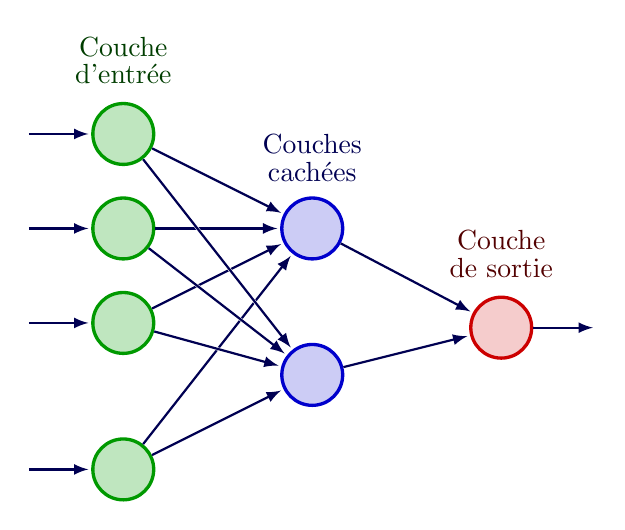
\begin{tikzpicture}[x=2.4cm,y=1.2cm]
    \readlist\Nnod{4,2,1} % array of number of nodes per layer
    \readlist\Nstr{n,m,k} % array of string number of nodes per layer
    \readlist\Cstr{x,h^{(\prev)},y} % array of coefficient symbol per layer
    \def\yshift{0.55} % shift last node for dots

    % LOOP over LAYERS
    \foreachitem \N \in \Nnod{

        \def\lay{\Ncnt} % alias of index of current layer
        \pgfmathsetmacro\prev{int(\Ncnt-1)} % number of previous layer
        \foreach \i [evaluate={\c=int(\i==\N); \y=\N/2-\i-\c*\yshift;
                    \x=\lay; \n=\nstyle;
                    \index=(\i<\N?int(\i):"\Nstr[\n]");}] in {1,...,\N}{ % loop over nodes
                % NODES
                % \node[node \n] (N\lay-\i) at (\x,\y) {$\strut\Cstr[\n]_{\index}$};
                \node[node \n] (N\lay-\i) at (\x,\y) {};

                % CONNECTIONS
                \ifnumcomp{\lay}{>}{1}{ % connect to previous layer
                    \foreach \j in {1,...,\Nnod[\prev]}{ % loop over nodes in previous layer
                            \draw[white,line width=1.2,shorten >=1] (N\prev-\j) -- (N\lay-\i);
                            \draw[connect] (N\prev-\j) -- (N\lay-\i);
                        }
                    \ifnum \lay=\Nnodlen
                        \draw[connect] (N\lay-\i) --++ (0.5,0); % arrows out
                    \fi
                }{
                    \draw[connect] (0.5,\y) -- (N\lay-\i); % arrows in
                }

            }
        % \path (N\lay-\N) --++ (0,1+\yshift) node[midway,scale=1.6] {$\vdots$}; % dots
    }
    
    % LABELS
    \node[above=3,align=center,mydarkgreen] at (N1-1.90) {Couche\\[-0.2em]d'entrée};
    \node[above=2,align=center,mydarkblue] at (N2-1.90) {Couches\\[-0.2em]cachées};
    \node[above=3,align=center,mydarkred] at (N\Nnodlen-1.90) {Couche\\[-0.2em]de sortie};

\end{tikzpicture}


\end{document}